\documentclass{article}
\usepackage{graphicx} % For including images
\usepackage{amsmath}  % For mathematical equations
\usepackage{amssymb}  % For mathematical symbols
\usepackage{hyperref} % For hyperlinks
\usepackage{geometry} % For adjusting page margins
\usepackage{booktabs} % For better table formatting
\usepackage{subcaption} % Add this package for subfigure support

\geometry{a4paper, margin=1in}

\title{Statistical Analysis of Deepfake Images and Videos in Smart City Applications}
\author{ANAND M K }
\date{242CS008}

\begin{document}

\maketitle

\section{Introduction}
Deepfake technology, which uses advanced machine learning algorithms such as generative adversarial networks (GANs), has made it possible to create highly realistic but entirely synthetic media, including images, videos, and audio. While deepfakes have a range of creative applications, they also present significant risks, particularly in sensitive areas where the authenticity of media is crucial. One such area is the functioning of smart cities, where a wide range of systems rely on media data for decision-making, including surveillance, traffic monitoring, and public safety mechanisms.

In this report, we focus on the statistical analysis of deepfake image and video datasets, specifically examining basic statistical measures such as the mean, median, and mode of pixel intensities. These measures, though simple, are fundamental in exploring the distribution of pixel values and identifying patterns that could indicate synthetic manipulation of media. By applying statistical methods to deepfake datasets, we aim to uncover the intrinsic properties of deepfake images and videos, such as unusual patterns in pixel intensity distributions, that might differentiate them from authentic media.

Additionally, this analysis will explore more advanced statistical techniques to analyze the variations in pixel intensities, including variance, skewness, and kurtosis. These higher-order statistical properties provide deeper insights into the structure and texture of media, potentially highlighting anomalies that are characteristic of deepfake images and videos. The goal is not to detect deepfakes directly but to understand their statistical behavior and identify patterns that may emerge from their generation.

The results of this analysis will provide valuable insights into the statistical characteristics of deepfake media and how these properties may impact data-driven decision-making in smart cities. Understanding these characteristics will help inform future studies and methodologies for dealing with synthetic media in urban environments, ensuring that media used in smart city systems is both reliable and representative of the real world.

By examining deepfake datasets through the lens of statistical analysis, this study contributes to a more nuanced understanding of how statistical measures can be used to analyze and understand synthetic media, laying the foundation for more informed approaches to handling media data in smart cities.

\newpage

\section{Datasets Used}
The following datasets were used for the experiments:

\begin{itemize}
    \item \textbf{FaceForensics}: A large-scale dataset containing real and manipulated videos, focusing on deepfake detection.
    \item \textbf{OpenForensics}: A dataset designed for forensic analysis, including real and synthetic images.
    \item \textbf{UADFV}: A dataset containing real and deepfake videos, commonly used for deepfake detection research.
\end{itemize}

Below are sample images of one real and one fake (deepfake) image from the datasets:

\begin{figure}[h!]
    \centering
    \begin{subfigure}{0.45\textwidth}
        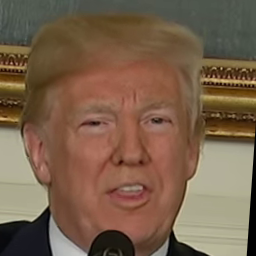
\includegraphics[width=\textwidth]{real.png}
        \caption{Real Image}
        \label{fig:real_image}
    \end{subfigure}
    \hfill
    \begin{subfigure}{0.45\textwidth}
        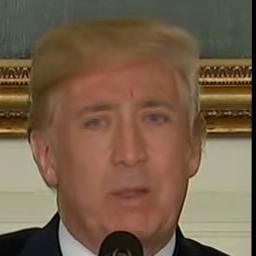
\includegraphics[width=\textwidth]{fake.png}
        \caption{Fake (Deepfake) Image}
        \label{fig:fake_image}
    \end{subfigure}
    \caption{Sample images: Real and Fake (Deepfake) from the datasets.}
    \label{fig:sample_images}
\end{figure}


\section{Descriptive Statistics}
Descriptive statistics refers to a set of techniques used to summarize and describe the main features of a dataset. It provides simple summaries about the sample and the measures, such as central tendency (mean, median, mode), variability (variance, standard deviation), and distribution (histograms). These methods help in understanding the basic characteristics of the data, making it easier to interpret and analyze.

\subsection{Mean, Median, and Mode of Pixel Intensities}
The mean, median, and mode are measures of central tendency that describe the average, middle, and most frequent pixel intensity values in an image, respectively.

\begin{table}[h!]
    \centering
    \begin{tabular}{lccc}
        \toprule
        \textbf{Image Type} & \textbf{Mean} & \textbf{Median} & \textbf{Mode} \\
        \midrule
        Real Image & 101.221 & 95.0 & 84 \\
        Deepfake Image & 94.787 & 91.0 & 0 \\
        \bottomrule
    \end{tabular}
    \caption{Mean, Median, and Mode of Pixel Intensities}
    \label{tab:mean_median_mode}
\end{table}

\subsection{Variance and Standard Deviation of Pixel Values}
Variance and standard deviation measure the spread of pixel intensity values around the mean. Variance is the average of the squared differences from the mean, while standard deviation is the square root of variance.

\begin{table}[h!]
    \centering
    \begin{tabular}{lcc}
        \toprule
        \textbf{Image Type} & \textbf{Variance} & \textbf{Standard Deviation} \\
        \midrule
        Real Image & 1392.574 & 37.317 \\
        Deepfake Image & 1902.004 & 43.612 \\
        \bottomrule
    \end{tabular}
    \caption{Variance and Standard Deviation of Pixel Values}
    \label{tab:variance_std}
\end{table}

\subsection{Histograms of Pixel Distributions}
A histogram represents the distribution of pixel intensities in an image. It shows the frequency of each intensity value.

\begin{figure}[h!]
    \centering
    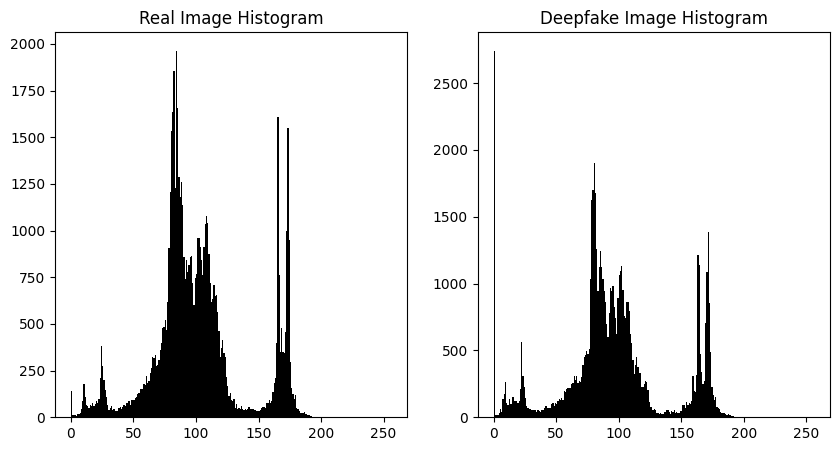
\includegraphics[width=0.8\textwidth]{histograms.png}
    \caption{Histograms of pixel distributions for real and deepfake images.}
    \label{fig:histograms}
\end{figure}

\subsection{Correlation Between Pixel Values}
Correlation measures the relationship between pixel values in different regions of an image. A value close to 1 indicates a strong positive correlation, while a value close to -1 indicates a strong negative correlation.

\begin{table}[h!]
    \centering
    \begin{tabular}{lc}
        \toprule
        \textbf{Image Type} & \textbf{Correlation} \\
        \midrule
        Real Image & -0.038 \\
        Deepfake Image & 0.171 \\
        \bottomrule
    \end{tabular}
    \caption{Correlation Between Pixel Values}
    \label{tab:correlation}
\end{table}

\subsection{Temporal Statistics for Videos}
Temporal statistics analyze frame-by-frame changes in pixel intensity for videos. This helps in understanding the dynamics of pixel intensity over time.

\begin{figure}[h!]
    \centering
    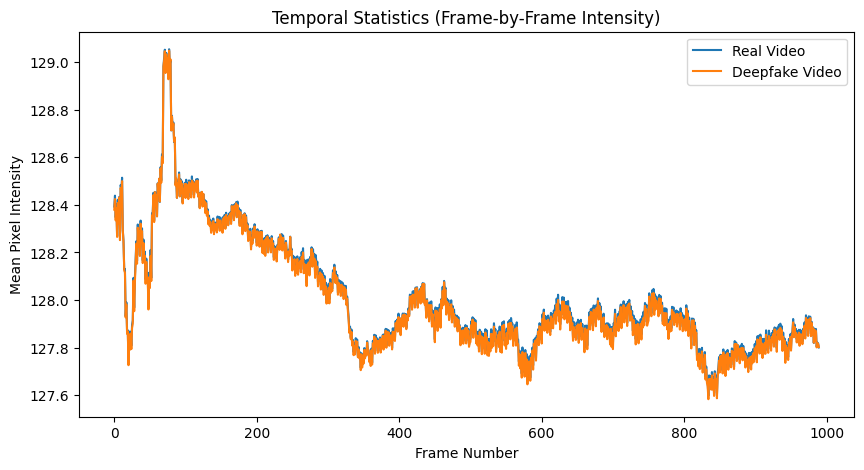
\includegraphics[width=0.8\textwidth]{temporal_statistics.png}
    \caption{Temporal statistics (frame-by-frame intensity changes) for real and deepfake videos.}
    \label{fig:temporal}
\end{figure}

\section{Feature Extraction Statistics}
Feature extraction is a crucial step in image and video analysis, allowing us to obtain meaningful patterns and characteristics from the data. Various methods are applied to analyze texture, edges, frequency components, and motion to distinguish between real and deepfake media. This section presents the results of applying multiple feature extraction techniques to both real and deepfake images and videos.

\subsection{Canny Edge Detection}
Canny edge detection is a multi-stage algorithm used to detect edges in an image. It applies:
\begin{enumerate}
    \item A Gaussian filter to smooth the image and reduce noise.
    \item Gradient computation to identify intensity changes.
    \item Non-maximum suppression to thin out edges.
    \item Hysteresis thresholding to detect strong and weak edges.
\end{enumerate}
This method is effective for highlighting boundaries and structural features in an image.

\begin{figure}[h!]
    \centering
    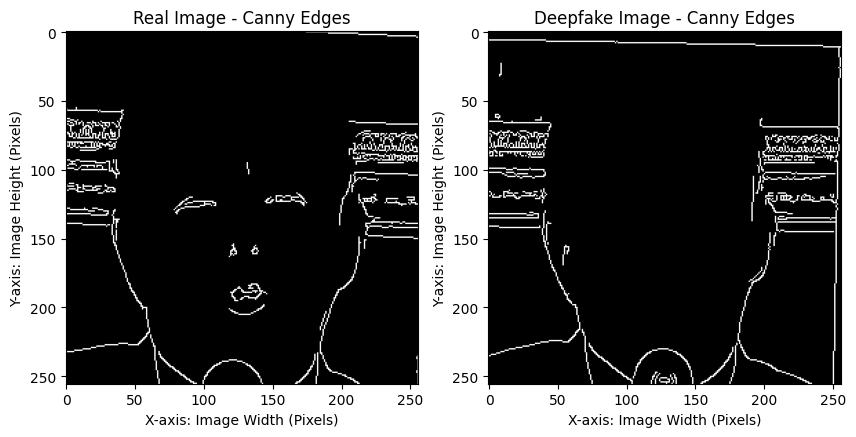
\includegraphics[width=0.8\textwidth]{real_canny.png}
    \caption{Real Image - Canny Edge Detection}
    \label{fig:real_canny}
\end{figure}

\subsection{Haralick Features}
Haralick features are texture features derived from the Gray-Level Co-occurrence Matrix (GLCM). These features capture statistical properties of texture, including:
\begin{enumerate}
    \item \textbf{Contrast:} Measures the intensity difference between adjacent pixels.
    \item \textbf{Correlation:} Describes the degree of similarity between neighboring pixels.
    \item \textbf{Energy:} Indicates uniformity in texture patterns.
    \item \textbf{Homogeneity:} Measures how uniform the intensity distribution is.
\end{enumerate}
Haralick features are widely used in texture classification and image analysis.

\begin{table}[h]
    \centering
    \begin{tabular}{|c|c|c|}
        \hline
        \textbf{Feature} & \textbf{Real Image} & \textbf{Deepfake Image} \\
        \hline
        Contrast & 57.7027 & 104.8085 \\
        Correlation & 0.9793 & 0.9723 \\
        Energy & 0.0540 & 0.0693 \\
        Homogeneity & 0.4950 & 0.5452 \\
        \hline
    \end{tabular}
    \caption{Haralick Features for Real and Deepfake Images}
    \label{tab:haralick_features}
\end{table}

\subsection{Sobel Edge Detection}
The Sobel operator detects edges by computing intensity gradients at each pixel. It enhances regions with high spatial frequency, making edges more pronounced.

\begin{figure}[h!]
    \centering
    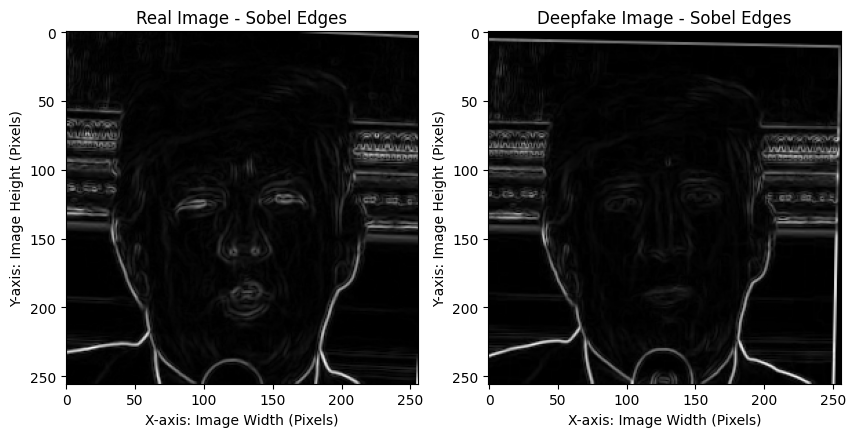
\includegraphics[width=0.8\textwidth]{real_sobel.png}
    \caption{Real Image - Sobel Edge Detection}
    \label{fig:real_sobel}
\end{figure}

\subsection{Local Binary Patterns (LBP)}
Local Binary Patterns (LBP) encode texture by comparing each pixel with its neighbors:
\begin{enumerate}
    \item Taking a pixel and comparing it to its neighbors.
    \item Assigning binary values based on whether a neighboring pixel is brighter or darker.
    \item Converting the binary pattern into a decimal value for classification.
\end{enumerate}
LBP is useful for identifying patterns in textures, such as in facial recognition and material classification.

\begin{figure}[h!]
    \centering
    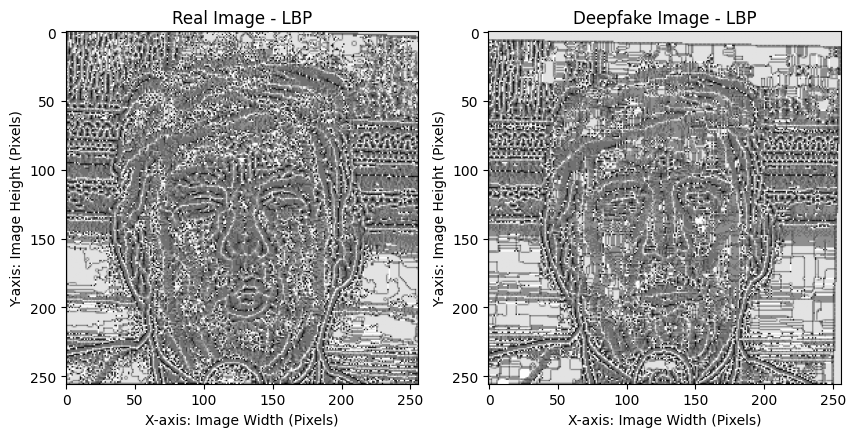
\includegraphics[width=0.8\textwidth]{real_lbp.png}
    \caption{Real Image - Local Binary Patterns}
    \label{fig:real_lbp}
\end{figure}

\subsection{Fourier Transform}
The Fourier Transform decomposes an image into its frequency components. It is useful for:
\begin{enumerate}
    \item Identifying periodic patterns in textures.
    \item Filtering noise and unwanted frequency components.
    \item Analyzing frequency-based features in images.
\end{enumerate}

\begin{figure}[h!]
    \centering
    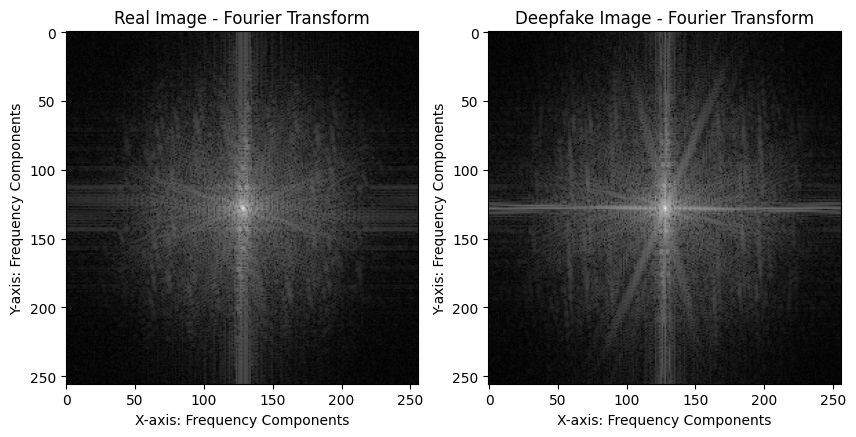
\includegraphics[width=0.8\textwidth]{real_fourier.png}
    \caption{Real Image - Fourier Transform}
    \label{fig:real_fourier}
\end{figure}

\subsection{Wavelet Transform}
The Wavelet Transform decomposes an image into different frequency sub-bands, providing both spatial and frequency information. It breaks an image into:
\begin{enumerate}
    \item \textbf{Approximation (cA):} Represents low-frequency components.
    \item \textbf{Horizontal Detail (cH):} Highlights horizontal edges.
    \item \textbf{Vertical Detail (cV):} Highlights vertical edges.
    \item \textbf{Diagonal Detail (cD):} Captures diagonal edge information.
\end{enumerate}

\begin{figure}[h!]
    \centering
    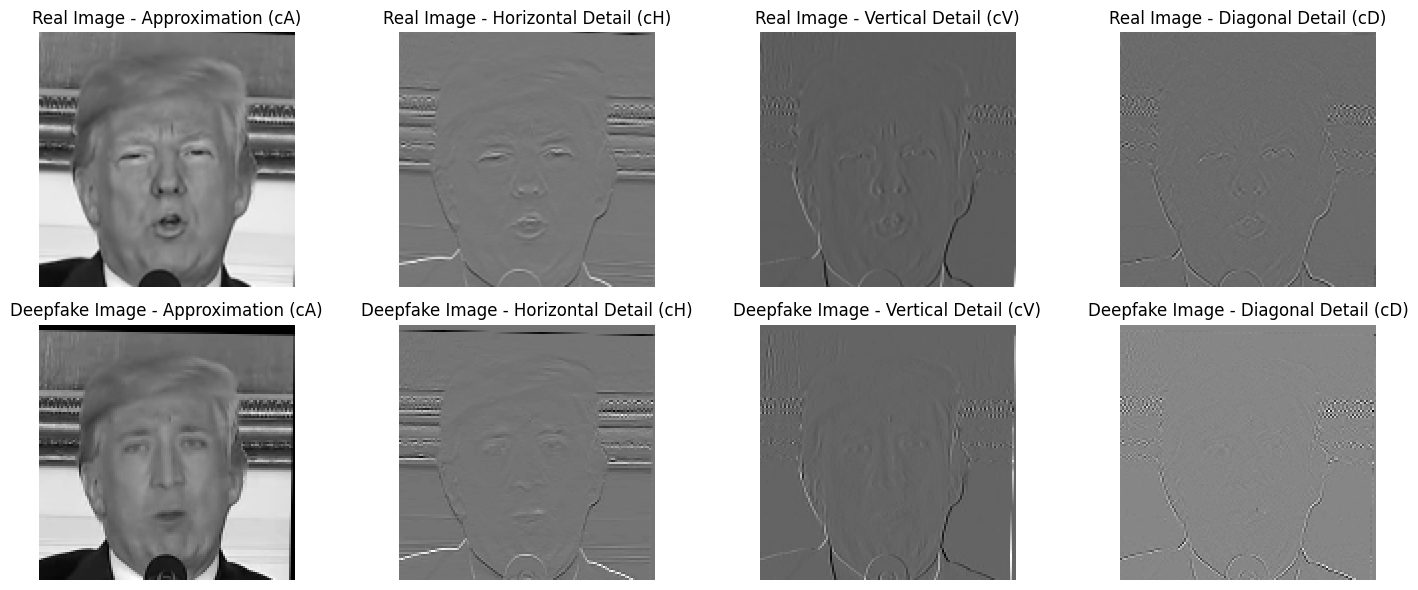
\includegraphics[width=1\textwidth]{real_wavelet_cA.png}
    \caption{Real Image - Wavelet Transform Approximation (cA)}
    \label{fig:real_wavelet_cA}
\end{figure}

\subsection{Average Frame Difference}
The average frame difference method calculates pixel intensity changes between consecutive frames in a video. It helps detect motion and temporal inconsistencies, useful in:
\begin{enumerate}
    \item Identifying scene changes and motion intensity.
    \item Analyzing temporal consistency in real vs. deepfake videos.
    \item Spotting unusual changes that could indicate manipulation.
\end{enumerate}

\begin{figure}[h!]
    \centering
    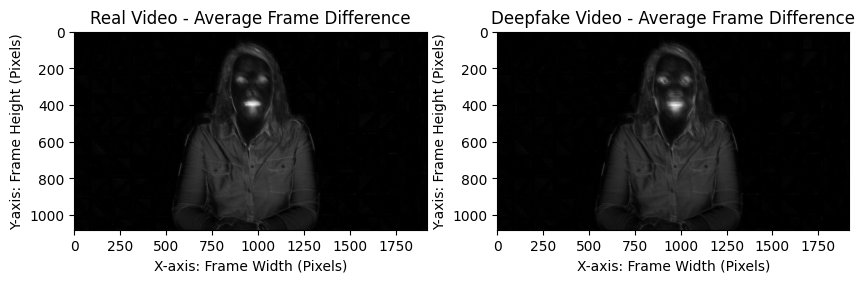
\includegraphics[width=1\textwidth]{real_avg_diff.png}
    \caption{Real Video - Average Frame Difference}
    \label{fig:real_avg_diff}
\end{figure}


\section{Statistical Modeling Methods}

This section explores the application of statistical modeling techniques to analyze real and deepfake images and videos. The methods used include Gaussian Mixture Models (GMM) for image analysis and Hidden Markov Models (HMM) for video analysis. These models help in understanding the underlying statistical properties and temporal patterns of real and deepfake data.

\subsection{Gaussian Mixture Models (GMM)}
Gaussian Mixture Models (GMM) are probabilistic models used to represent the distribution of pixel intensities in images. By fitting a mixture of Gaussian distributions to the image pixels, we can analyze their statistical properties and detect patterns that distinguish real and deepfake images.


\begin{figure}[h]
\centering
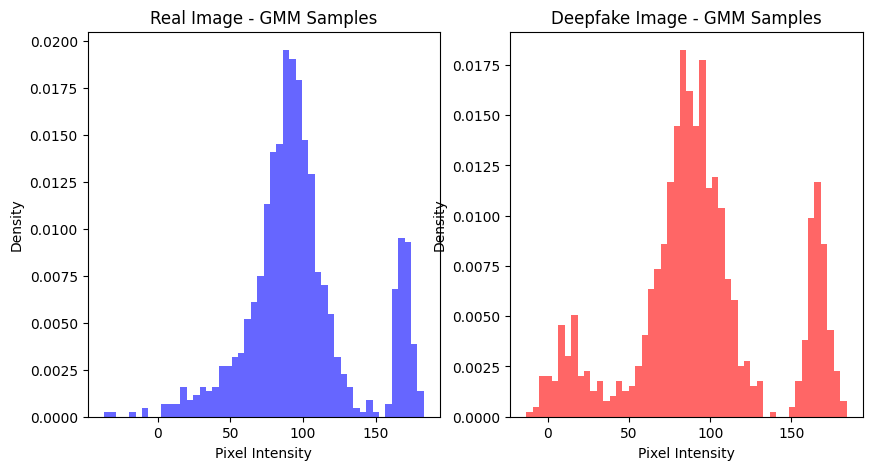
\includegraphics[width=1\textwidth]{gmm_results.png}
\caption{GMM Pixel Intensity Distributions for Real and Deepfake Images}
\label{fig:gmm_results}
\end{figure}

\subsection{Hidden Markov Models (HMM)}
Hidden Markov Models (HMM) are used to analyze temporal sequences, such as frame-by-frame changes in videos. By modeling the progression of pixel intensities across frames, HMM helps in identifying patterns that differentiate real and deepfake videos.


\begin{figure}[h]
\centering
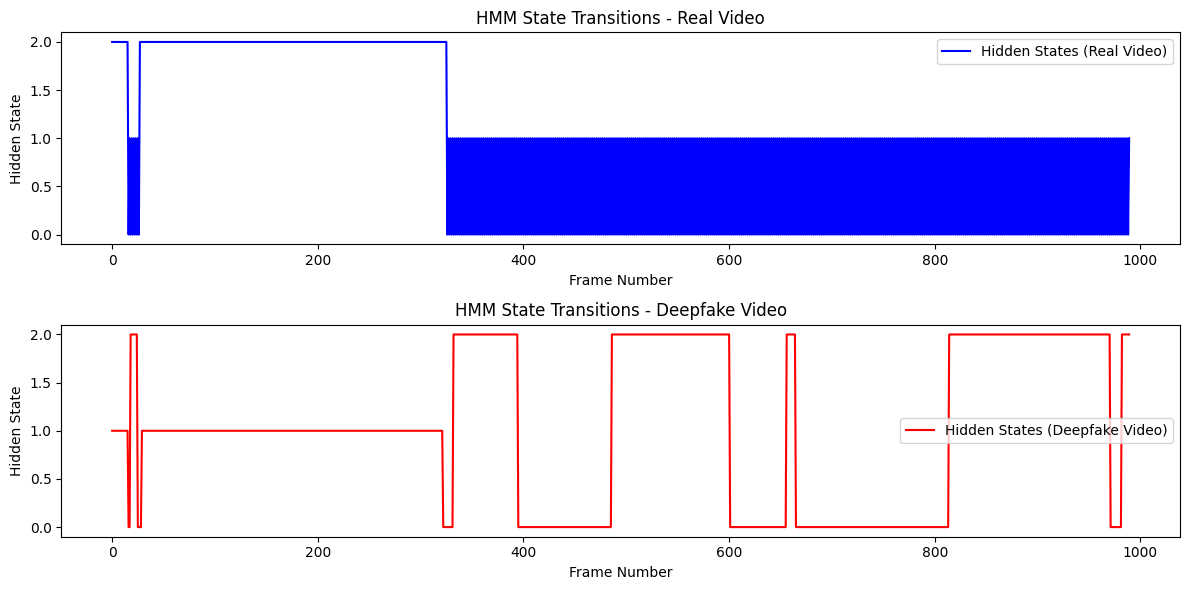
\includegraphics[width=1\textwidth]{hmm_results.png}
\caption{HMM State Transitions for Real and Deepfake Videos}
\label{fig:hmm_results}
\end{figure}

\section{Statistical Tools for Analyzing Deepfake Images and Videos}

\subsection{OpenCV (Open Source Computer Vision Library)}
\textbf{OpenCV} is a widely-used open-source computer vision library. It provides several statistical methods that can be applied to deepfake image and video analysis:
\begin{itemize}
    \item \textbf{Histogram Analysis}: Statistical comparison of color histograms to find discrepancies in pixel distribution between real and deepfake images.
    \item \textbf{Optical Flow Analysis}: Optical flow algorithms track the movement of objects across video frames, which can help identify inconsistencies in motion patterns typical of deepfakes.
    \item \textbf{Edge Detection}: OpenCV provides tools like the Canny edge detector that can reveal subtle inconsistencies in deepfake images by analyzing edge features.
\end{itemize}

\subsection{Scikit-Image}
\textbf{Scikit-Image} is a Python library for image processing, built on top of Scikit-learn. It offers a variety of statistical tools for image analysis:
\begin{itemize}
    \item \textbf{Texture Analysis}: Local Binary Patterns (LBP) and other texture features can be used to detect statistical differences between real and fake textures.
    \item \textbf{Statistical Image Measures}: Tools to calculate entropy, skewness, and kurtosis of pixel distributions, which can expose unnatural patterns that deepfakes often introduce.
\end{itemize}

\subsection{Matlab and Image Processing Toolbox}
\textbf{Matlab} is a high-performance language for technical computing, and its Image Processing Toolbox offers several statistical techniques:
\begin{itemize}
    \item \textbf{Fourier Transform}: Fourier analysis of the frequency domain to reveal inconsistencies in the deepfake’s pixel composition that wouldn't occur in natural images.
    \item \textbf{Fractal Dimension Analysis}: This statistical method measures the complexity of textures in images and can be used to detect anomalies in deepfakes.
    \item \textbf{Principal Component Analysis (PCA)}: PCA reduces the dimensionality of image data and reveals the key features, helping identify statistical differences between real and deepfake media.
\end{itemize}

\subsection{PyTorch and TensorFlow}
\textbf{PyTorch} and \textbf{TensorFlow} are deep learning frameworks that can be used for custom models to perform statistical analysis on deepfake media:
\begin{itemize}
    \item \textbf{Residual Analysis}: Statistical analysis of the difference between predicted (realistic) and actual deepfake images/videos.
    \item \textbf{Discrepancy in Feature Distribution}: Models can be trained to focus on features like textures, motion, or edges in videos, and statistical tests can highlight differences between real and manipulated data.
\end{itemize}

\subsection{NumPy and SciPy}
\textbf{NumPy} and \textbf{SciPy} are fundamental libraries for scientific computing in Python. They offer functions for:
\begin{itemize}
    \item \textbf{Mean, Standard Deviation, and Variance}: Basic statistical operations to analyze pixel intensities across images or video frames.
    \item \textbf{Correlation Coefficients}: Compute pixel correlations across regions to find inconsistencies in deepfake images or videos.
    \item \textbf{Statistical Clustering}: Methods like k-means clustering can be used to group image pixels and analyze statistical differences between real and fake images.
\end{itemize}

\section*{Conclusion}
In this study, various statistical methods were applied to analyze real and deepfake images and videos. Descriptive statistics, including mean, median, variance, and histograms, provided insights into pixel intensity distributions. Feature extraction techniques, such as edge detection, texture analysis, and frequency domain transformations (Fourier and Wavelet), highlighted structural differences between real and manipulated content. Statistical modeling using Gaussian Mixture Models (GMM) and Hidden Markov Models (HMM) further captured the underlying distributions and temporal dynamics of the data. Tools like OpenCV, Scikit-Learn, and HMMLearn, along with datasets such as FaceForensics++ and DFDC, were instrumental in implementing these methods. The results demonstrated significant differences in pixel intensity, texture, and temporal patterns, offering a foundation for robust deepfake detection systems. Future work could integrate deep learning models and explore larger datasets to enhance detection accuracy and real-time applicability. Overall, this study underscores the effectiveness of statistical methods in understanding and combating deepfake media.


\end{document}
